Little introduction: 
\begin{itemize}
    \item Experimental and theoretical physicist, was the old distinction
    \item The different categories of astronomy
    \item The uniqueness of a computational astrophysicist
    \item What is the job of a computational astrophysicist
    \item How a computational astrophysicist is doing a “theoretical experiment”
    \item How this thesis fits in that 
\end{itemize}


\section{The Explicit Physics}
    My simulations solve the \textit{restricted three body problem}. In essence
    \begin{figure}
        \centering
        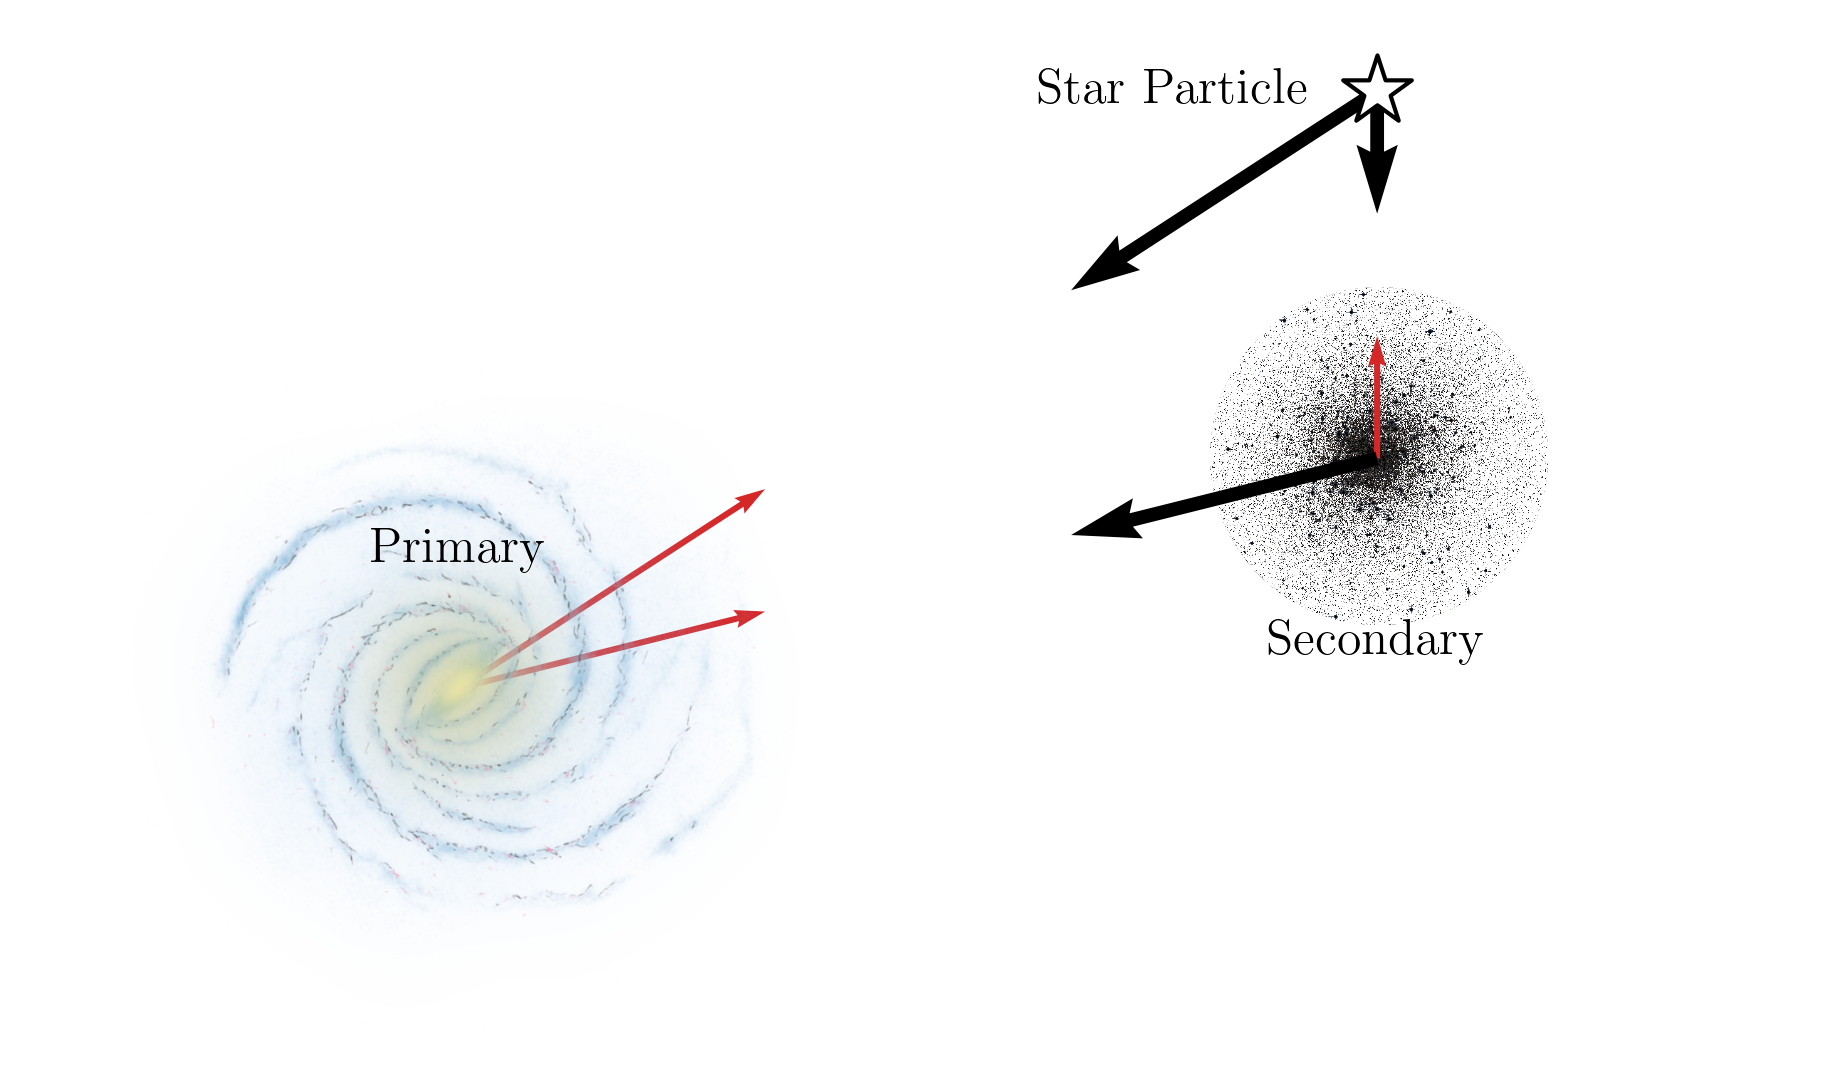
\includegraphics[width=\linewidth]{images/restricted_three_body_set_up.png}
        \caption{Little sketch of my equations of motion. }
    \end{figure}
    
    \subsection{Equations of Motion} \label{subsec:myEquationsOfMotion}
        I like to start with the \textit{Lagrangian}, which comes from the variational principle which states that particles with move along trajectories that minimize the difference, $ L = T-U $, which $L$ is the Lagrangian, $T$ is the kinetic energy and $U$ is the potential energy. Also, as is almost always the case in gravitational dynamics, we normalize by the mass and use \textit{specific} energy: 
        \begin{equation}
            \mathcal{L} = \frac{L}{m} = \frac{1}{2}\left(\dot{x}^2+\dot{y}^2+\dot{z}^2\right) - \Phi(x,y,z).
        \end{equation}
        However, Lagrange's equations give a system of three second order coupled ordinary differential equations. If we switch to Hamiltonain dynamics, we can object a set of six \textit{first} order ordinary differential equations, which is easier to implement computationally. Also, since we are using the specific energy, the momentum coordinates for Hamilton's equations are the same as the velocities from the Lagrangian: $ p_i = \frac{\partial \mathcal{L}}{\partial \dot{q}_i}$. Therefore, $p_i = \dot{q}_i$, where $i \in \left(x,y,z\right)$. The Hamilton is derived through the Legendre transform: $ \mathcal{H}=\sum_i p_i\dot{q}_i - \mathcal{L}$. Then, we can apply Hamilton's equations to obtain the set of equations: 
        \begin{align}
            \dot{p}_i &= -\frac{\partial \mathcal{H}}{\partial q_i} \\
            \dot{q}_i &= \frac{\partial \mathcal{H}}{\partial p_i}
        \end{align}

        And when written explicity become: 
        \begin{align}
            \dot{p}_x &= -\frac{\partial \Phi}{\partial x} \\
            \dot{p}_y &= -\frac{\partial \Phi}{\partial y} \\
            \dot{p}_z &= -\frac{\partial \Phi}{\partial z} \\
            \dot{x} &= p_x \\ 
            \dot{y} &= p_y \\ 
            \dot{z} &= p_z \\ 
        \end{align}        


        \subsubsection*{The Globular Cluster}
            In the case of the Globular Clusters, they only feel the Galaxy. So their Hamiltonian becomes: 
            % \begin{equation}

            % \end{equation}

        \subsubsection*{The Star Particles}

    \subsection{Potential density pairs}

        \begin{figure}
            \centering
            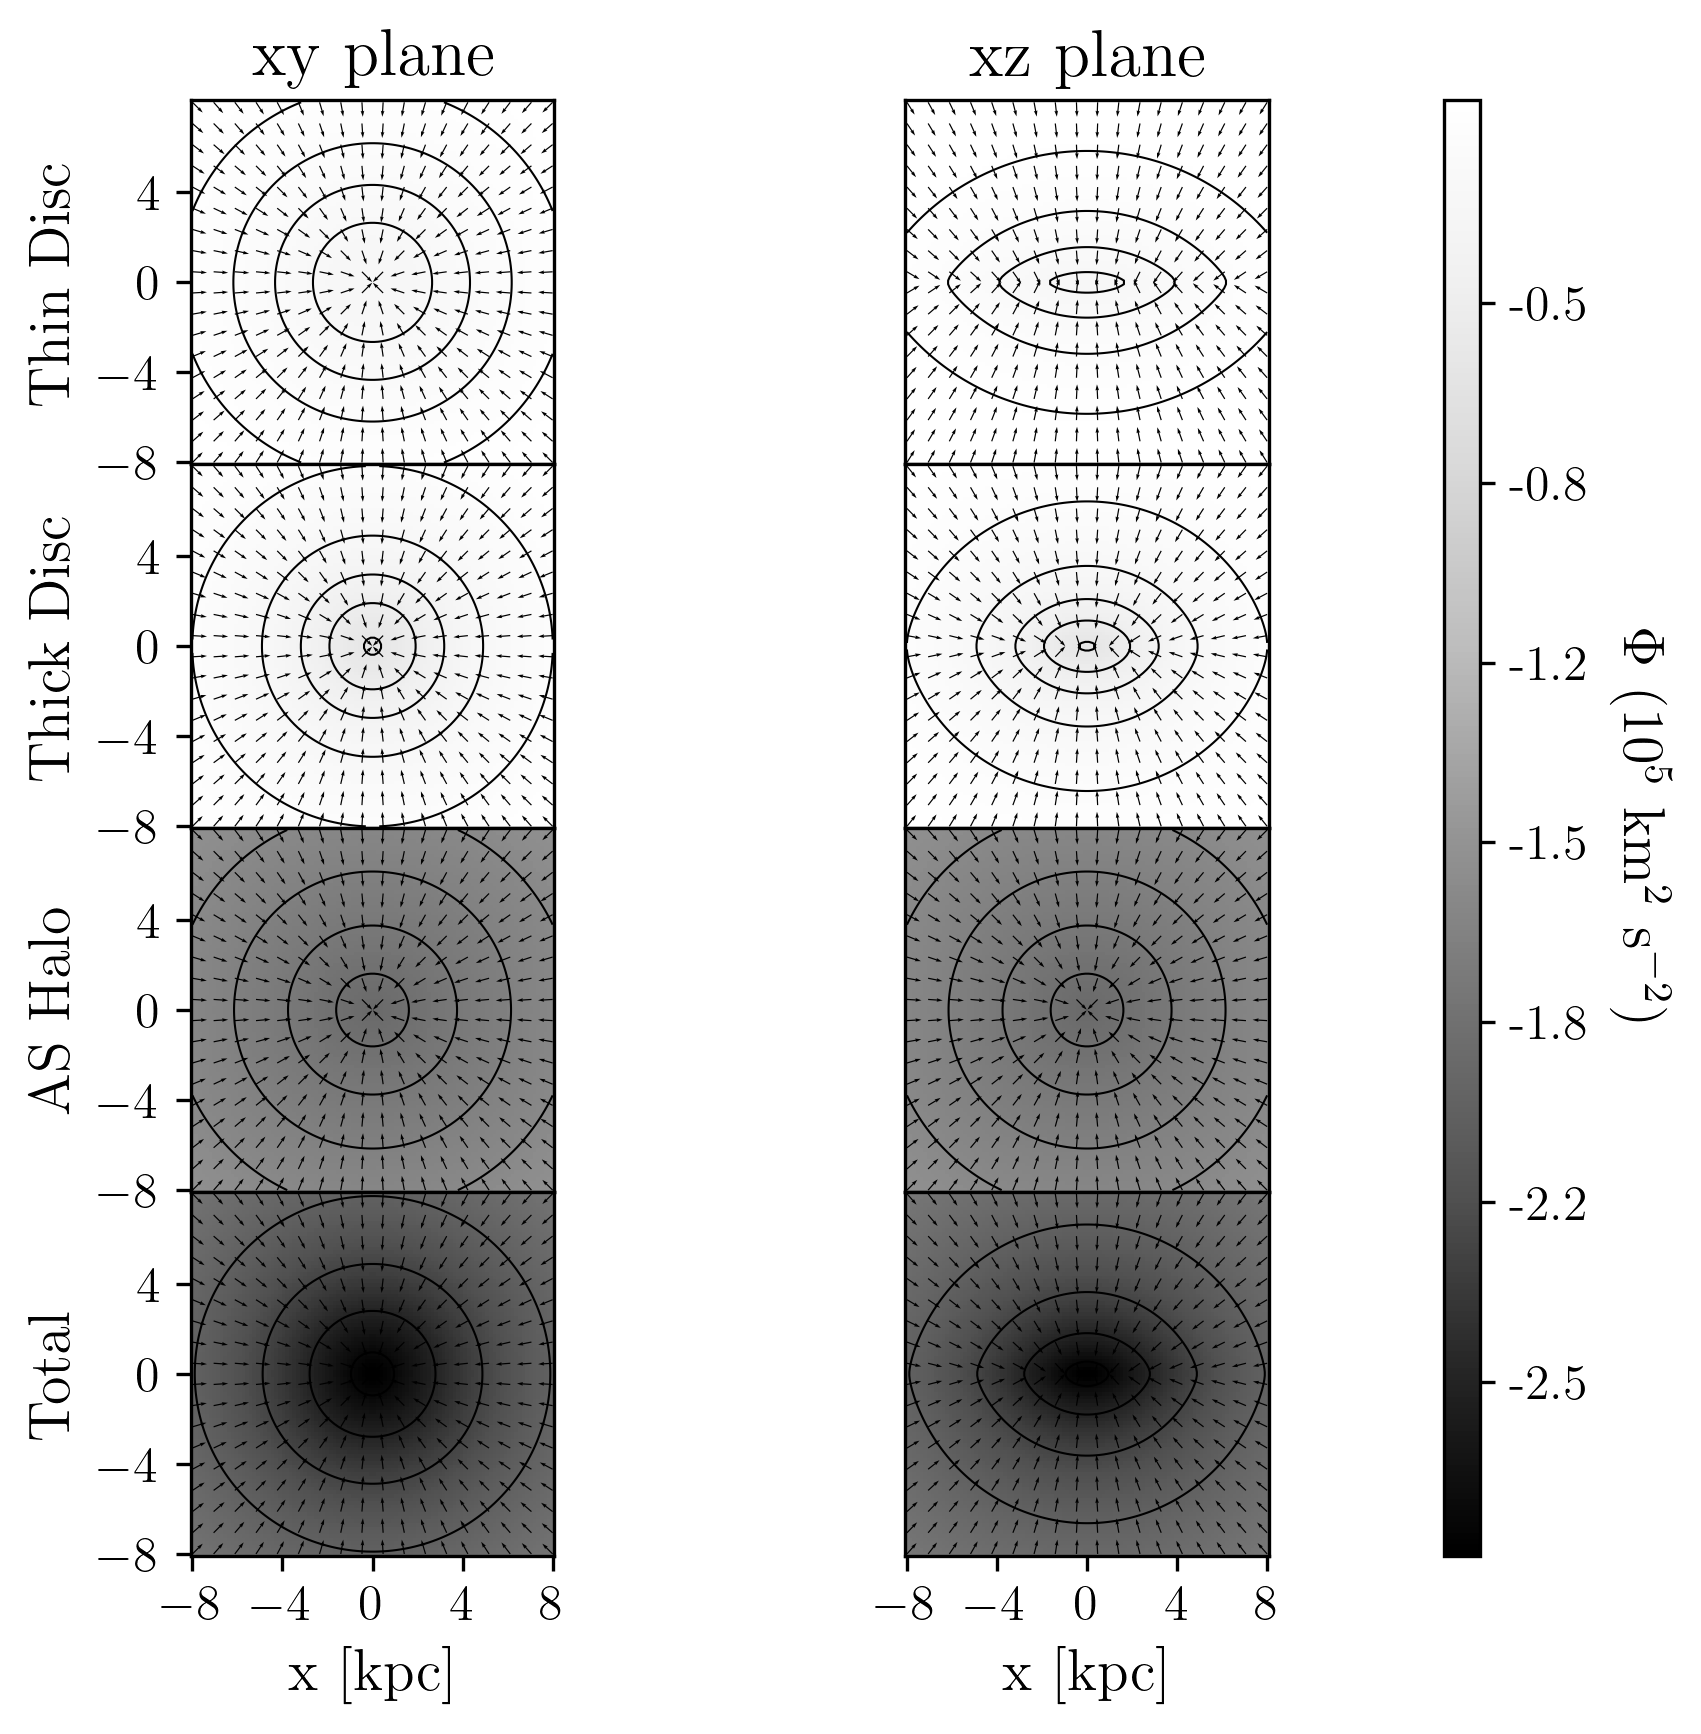
\includegraphics[width=\linewidth]{images/figure_pouliasis2017pii_potential_-8_8.png}
            \caption{The main potential used throughought the thesis}
        \end{figure}        
    

\section{The Implicit Physics}

    \subsection{The circular restricted three body problem}
        \begin{itemize}
            \item The Lagrange points
            \item Allowed regions 
        \end{itemize}

    \subsection{The tidal tensor}
        \begin{itemize}
            \item Either the Hessian of the Potential
            \item Or the Jacobian of the transform from position to force
            \item I prefer Jacobian
            \item We always use cartesian coordinates because if you do other systems, such as cylindrical or spherical, then you need to compute the cristoffer symbols. 
            \item Positive eigen values is stretching
            \item Negative eivenvalues is compression
            \item Stetching is a stronger deformation than compression
            \item For a spherical potential, the stretching deformation is parallel to the position vector. 
        \end{itemize}
        
        \begin{equation}
            \text{J}(F)= \left(\begin{matrix}
                \partial_x F_x & \partial_y F_x & \partial_z F_x \\
                \partial_x F_y & \partial_y F_y & \partial_z F_y \\
                \partial_x F_z & \partial_y F_z & \partial_z F_z 
            \end{matrix}\right)
        \end{equation}
        
        \subsubsection*{The Moon}


            \begin{itemize}
                \item If you talk about the tides, you have to start the conversation with the moon
                \item Cite the NASA website and say how many different ways we can evoke the tides
                \item since I do dynamics, I will discuss how the tides effect the orbit of the moon. 
                \item show with this little film that the tides slow down the orbit of the moon, make its distance wobble, and if you ignore it and only solve the 2 body problem + a rotating reference frame, after about 3/4 years you'll be completely off about your prediction.
                \item This is a cool point because the tides are even relevant on human time scales 
                \item There is no darkside of the moon. 
                \item cite the initial conditions from JPL
                \item Note that the drift of the moon from the earth is actually caused by the ocean and not the sun. Kinda crazy.
                \item Say this model is also an over simplification and that there's a whole field of study dedicated to all the librations of the moon with all the \textit{pertubations} from the simple two body problem. 
            \end{itemize}

            The tidal tensor for a keplerian potential: 
            \begin{equation}
                \mathcal{T}_{i,j}= \frac{GM_\odot}{r^3}\left(\begin{matrix}
                    1-\frac{3x^2}{r^2} & -\frac{3xy}{r^2} & -\frac{3xz}{r^2} \\
                    -\frac{3yx}{r^2} & 1-\frac{3y^2}{r^2} & -\frac{3yz}{r^2} \\
                    -\frac{3zx}{r^2} & -\frac{3zy}{r^2} & 1-\frac{3z^2}{r^2}
                \end{matrix}\right)
            \end{equation}            
\begin{verbatim}
VIDEO: moon_tidal_simulation.mp4
\end{verbatim}

            \begin{figure}
                \centering
                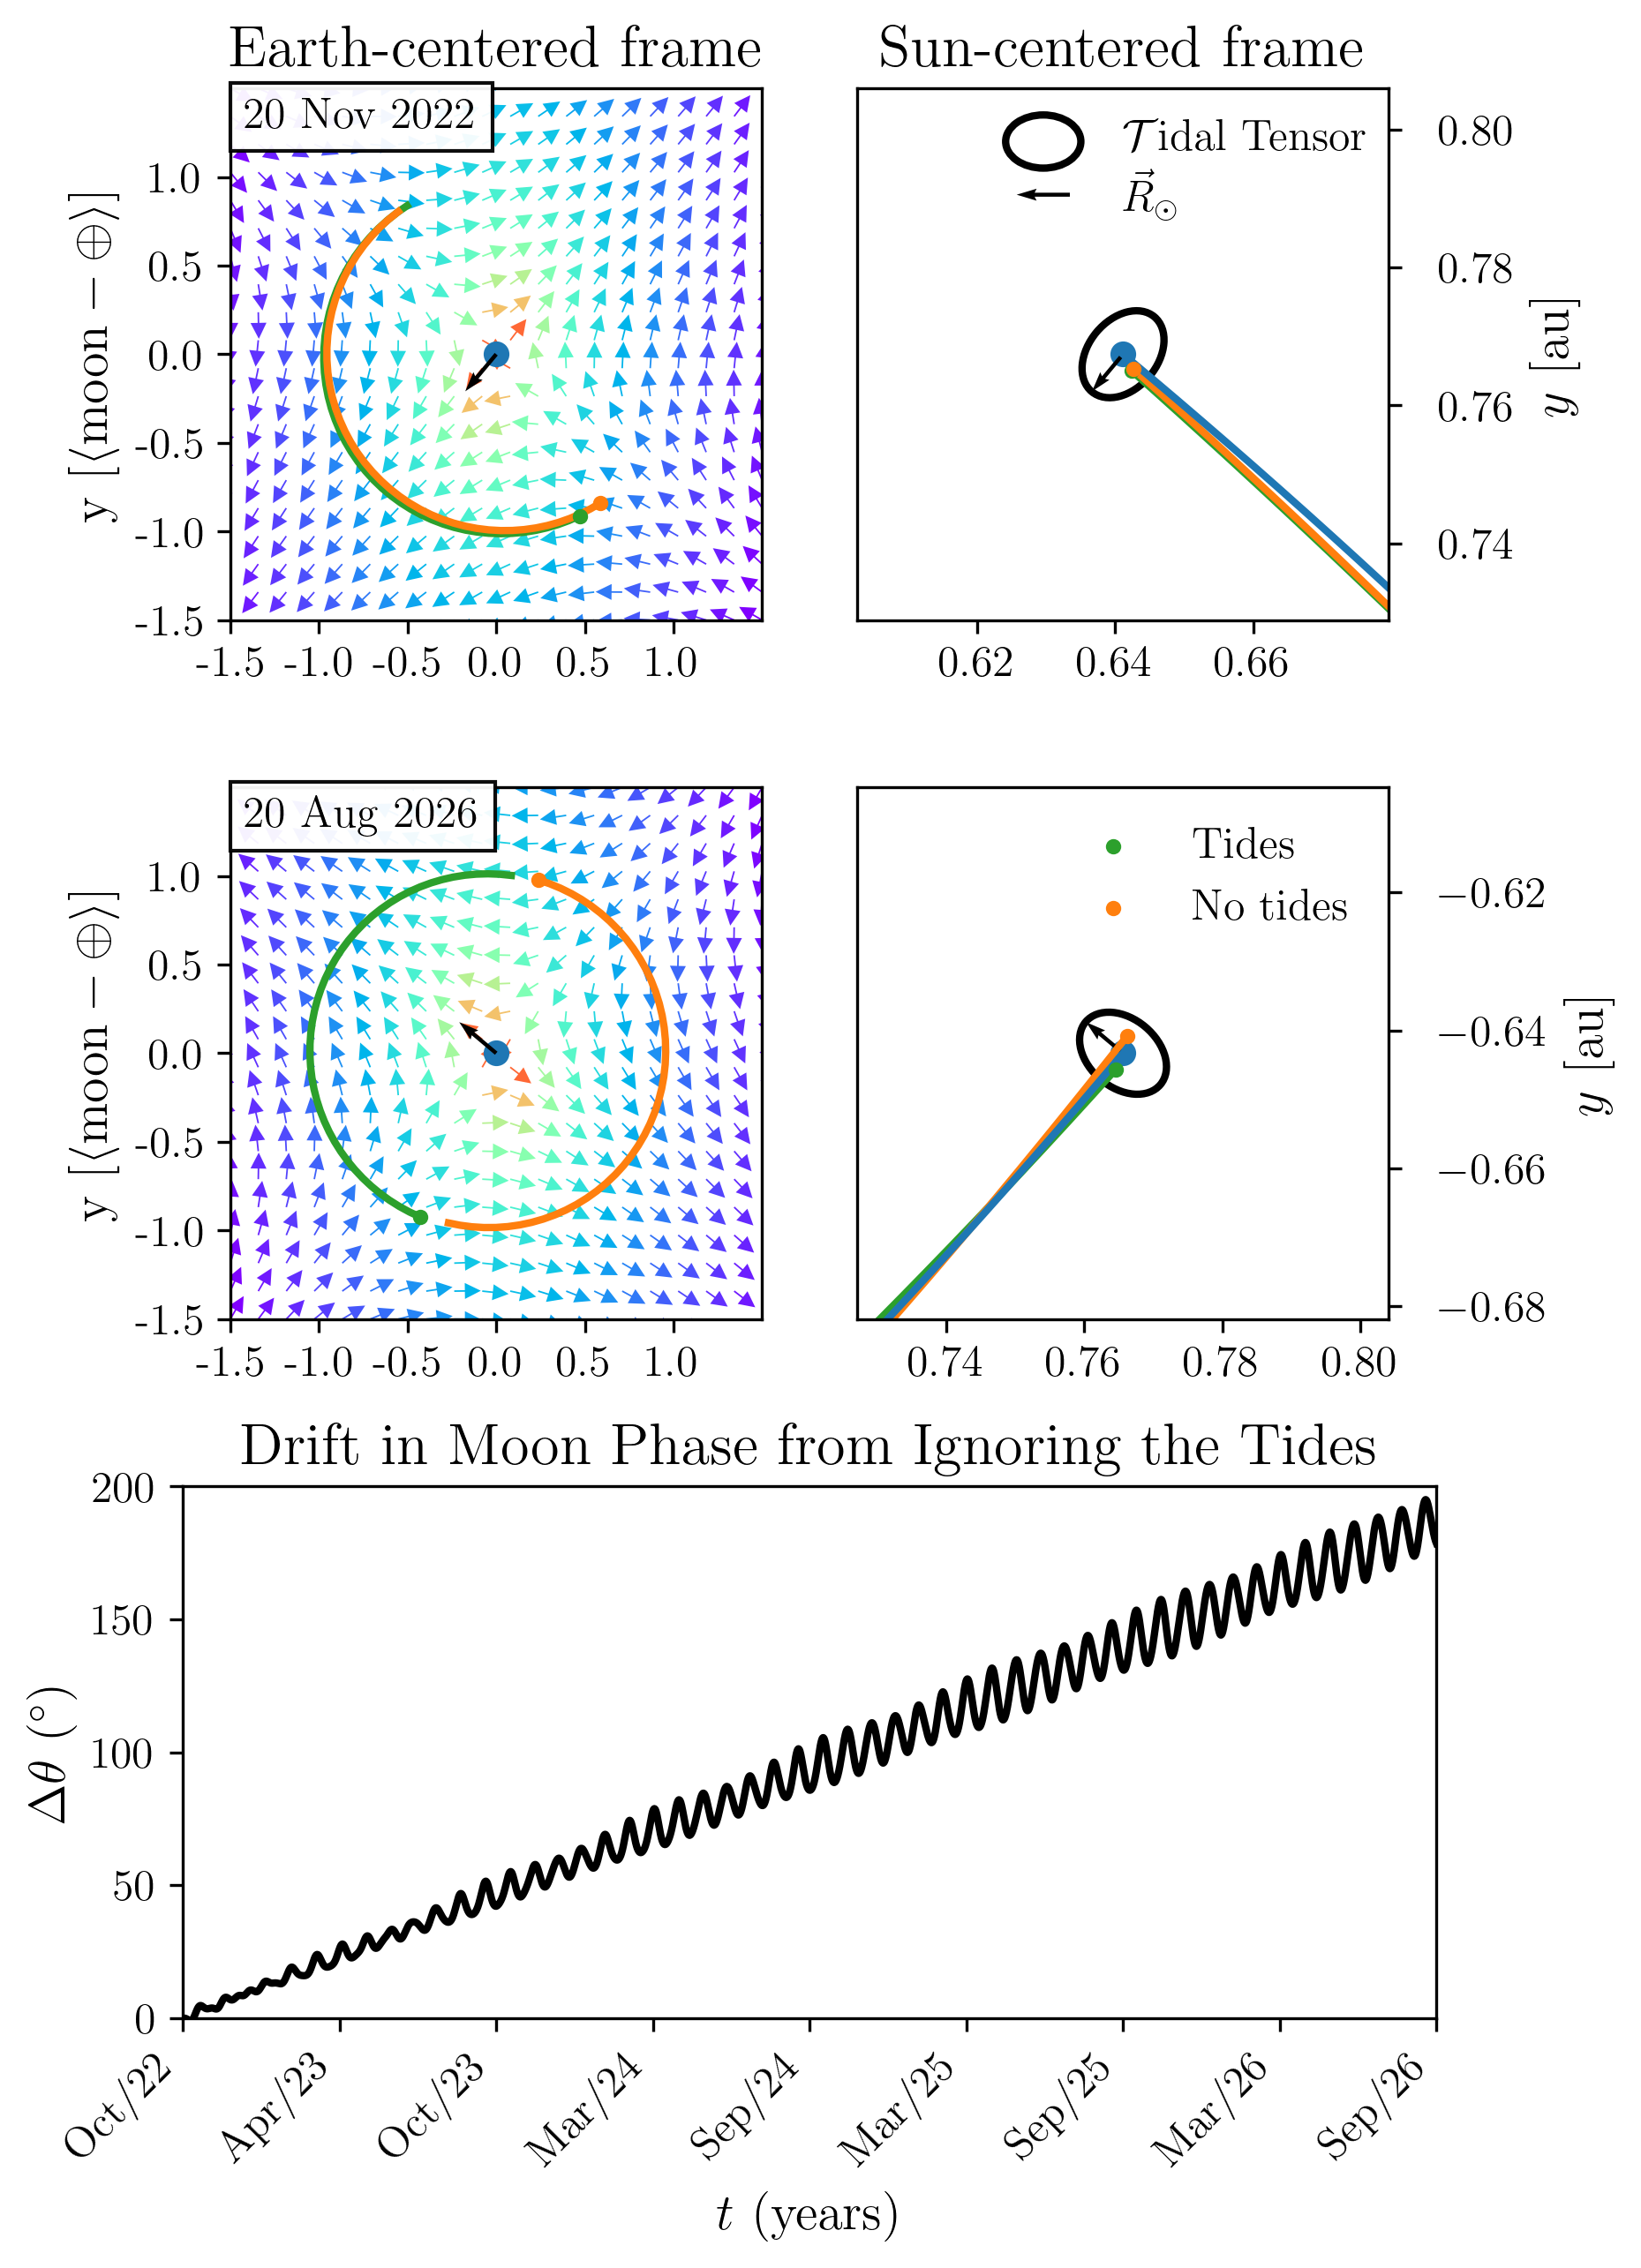
\includegraphics[width=\linewidth]{images/moon_tidal_simulation.png}
                \caption{The main potential used throughought the thesis}
            \end{figure}

        \subsubsection*{Tides in the Galaxy}
            \begin{itemize}
                \item Show some positions of the tidal tensor and how it can change orientation based on it's altitude 
                \item The tidal forces add together linearly, so show the Halo and the Disc example together. 
            \end{itemize}

            The Miyamoto Nagai potential is: 
            \begin{eqnarray}
                \Phi'   &= \frac{1}{D}\\
                D       &= \sqrt{x^2 + y^2 + \beta^2(z)}\\
                \beta(z)   &= 1 + \sqrt{z^2 + b^2}\\
                \beta'(z) &= \frac{z}{\sqrt{z^2 + b^2}}\\
                \beta''(z)  &= \frac{b^2}{\left(z^2 + b^2\right)^{3/2}}
            \end{eqnarray}

            The dimensionless tidal tensor then becomes: 

            \begin{equation}
                \mathcal{T}_{i,j}= \frac{1}{D^3}\left(\begin{matrix}
                    1-\frac{3x^2}{D^2} & -\frac{3xy}{D^2} & -\frac{3x\beta \beta'}{D^2} \\
                    \dots & 1-\frac{3y^2}{D^2} & -\frac{3y\beta \beta'}{D^2} \\
                    \dots & \dots & \beta'^2 + \beta \beta'' -\frac{3\left(\beta\beta'\right)^2}{D^2}
                \end{matrix}\right)
            \end{equation}    
            You can see immediately that multiplying the matrix by $\vec{v}=\lambda\left[x,y,z\right]$ does not return a vector that is parallel to the position vector, as it does for the spherical mass distribution. 

            The Marto's halo has this mass distribution:
            
            \begin{equation}
                M'_\text{enc}(s) = \frac{s^\gamma}{1+s^{\gamma-1}}
            \end{equation}
            The dimensionless tidal tensor is thus: 
            \begin{equation}
                \mathcal{T'}_{i,j}= \frac{M'_\text{enc}(s)}{s^3}\left(\begin{matrix}
                    1-\frac{x^2}{s^2}f(s) & -\frac{xy}{s^2}f(s) & -\frac{xz}{s^2}f(s) \\
                    -\frac{yx}{s^2}f(s) & 1-\frac{y^2}{s^2}f(s) & -\frac{yz}{s^2}f(s) \\
                    -\frac{zx}{s^2}f(s) & -\frac{zy}{s^2}f(s) & 1-\frac{z^2}{s^2}f(s)
                \end{matrix}\right)
            \end{equation}  
            where 
            \begin{equation}
                f(s) = 2-\frac{\gamma-1}{1+s^{\gamma-1}}
            \end{equation}

        \subsubsection*{Interesting case}
            There is a non-physical case that is extremely interesting. When you have a halo with a mass disrtibution that increases in density with distance, which is non-physical, the tidal tensor changes sign. This means that the strongest deformation is not longer stretching but squishing. I would like to do a stellar stream in this example. It would be fascinating. In this limit, the lagrange points should be on the sides of the stream instead of parallel to the position vector. 
            
            \begin{figure}
                \includegraphics[width=\linewidth]{images/martos_tidal_field_2_50_50.png}
                \caption{tidal field in normal martos potential }
            \end{figure}




    \subsection{Phase mixing}
        \begin{itemize}
            \item The Luiville theorem
            \item How it is slower with tidal tails 
            \item also the monte-carlo approach with phase mixing is what causes vast differences in orbital solutions after a certain period of time 
        \end{itemize}
    
    \subsection{Shocks}
        I started this section with the circular and planar restricted three body problem. It really simplifies the problem instead of looking for a general solution. All three bodies are point masses, in fact the tertiary body has no mass. The secondary is on a circular orbit about the primary, and the tertiary is in the same orbital plane as the secondary. This simplified problem is already quite complex but solvable and rich with physics. However, by restricting the orbits of the tertiary and secondary, we lose a lot of physics that affects our system. Additionally, for the globular clustres, most of them are not on circular orbits. Additionally, the galaxy is not a point mass, but rather a mass distribution with cylindrical symmetry.        



\section{The Ignored Physics}
    \subsection{Collisional dynamics}
        \begin{itemize}
            \item not nbody
            \item no mass segregation
            \item no three body encounters 
            \item no soft or hard binaries 
            \item show some results from Corespray 
        \end{itemize}
    
    \subsection{Stellar evolution}
        \begin{itemize}
            \item They're all point masses 
            \item No salpeter's 
            \item No strong initial mass loss 
            \item No accurate model for the colors 
            \item No multiple stellar populations 
        \end{itemize}
    
    \subsection{Time evolution}
        In someways, we take time evolution into account, and in someways, we ignore and this has already been covered in the previous sections. i.e., the orbit of the star-particles depend on the position of the host globular cluster, which I do not solve for simoltaneously but instead opt to load it into the computation, as shown in Section~\ref{subsec:myEquationsOfMotion}. Also, things like mass segregation and stellar evolution are time-dependent which is completely ignored in my simulations. 

